\section{Расширенный класс решений}
\subsection{Система уравнений для обобщённого кинетического уравнения}
\par Ранее рассмотренное кинетическое уравнение имело довольно простой вид, а именно $m_{t} = -u_{0}\gamma \alpha$, теперь мы попробуем придать ему более общий вид. Как отмечалось ранее, функция, характеризующая изменение пористости со временем, зависит от пористости в текущий момент времени. Пусть теперь кинетическое уравнение имеет вид $m_{t} = -F(m)\alpha$, где $F(m)$ --- произвольная функция. Перепишем нашу систему уравнеий:
\begin{equation*}
\begin{cases}

(m\alpha)_{t}+ u_{0}\alpha_{x} &= m_{t}\\
m_{t} &= -F(m)\alpha\\

\end{cases}
\end{equation*}

\par В отличие от рассмотренных до этого задач, мы перейдём не к переменной $\alpha$, а к переменной $m$. Пусть $\d G(m) = -\frac{1}{F(m)}$. Тогда
$$\Big(m \big(G(m)m_{t} - 1\big)\Big)_{t} + u_{0}\big(G(m)m_{t}\big)_{x} = 0$$

\par Докажем, что $\big(G m_{t}\big)_{x} = \big(G m_{x}\big)_{t}$.\\
\par Действительно, $\d \big(G(m)m_{t}\big)_{x} = G_{m}m_{t}m_{x} + G m_{tx} = \big(G m_{x}\big)_{t}$, откуда следует, что в нашем уравнении можно поменять местами производные по времени и по координате, а именно, получим:
$$\Big(m \big(G(m)m_{t} - 1\big)\Big)_{t} + u_{0}\big(G(m)m_{x}\big)_{t} = 0$$
\par Данное уравнение можно проинтегрировать по времени. Получим:\\
$$m \big(G(m)m_{t} - 1\big) + u_{0}G(m)m_{x} = \Phi(x)$$
где $\Phi(x)$ --- произвольная функция.
\par Переписывая последнее уравнение, получим:
$$m_{t}+\frac{u_{0}}{m}m_{x}=\frac{m+\Phi(x)}{G(m)m}$$
\par Это уравнение гиперболическое. Решая его методом характеристик, можем получить выражение для пористости.\\
\begin{equation*}
\begin{cases}

\d \frac{dm}{dt} &= \d \frac{m+\Phi(x)}{G(m)m}\\
&\\
\d \frac{dx}{dt}&= \d \frac{u_{0}}{m}\\
&\\
m_{t} &= -F(m)\alpha\\

\end{cases}
\end{equation*}

\par Решением одной из упрощённых задач было выражение для $m$. Обозначим
$$\d \theta=\frac{t-\frac{xm_{0}}{u_{0}}}{1 - \frac{\alpha_{0}-1}{\alpha_{0}}e^{\gamma x}}$$
\par Тогда:\\
$$m=m_{0}-\gamma u_{0}\theta$$
\par Найдём такую функцию $\Phi(x)$, которая соответствует данному решению. $G(m)=-\frac{1}{\gamma u_{0}}$. Для удобства выпишем, чему равны производные этого решения:\\
$$m = m_{0} - \gamma u_{0}\theta(t-\frac{xm_{0}}{u_{0}})$$
$$m_{t} = -\gamma u_{0}\theta$$
$$m_{x} = \gamma u_{0}\theta\frac{m_{0}}{u_{0}}-\gamma u_{0}(t-\frac{xm_{0}}{u_{0}})\theta^{2}\frac{\alpha_{0}-1}{\alpha_{0}}e^{\gamma x}\gamma$$\\
\par Подставляя и приводя подобные, получим $\Phi(x)=-m_{0}$.
\par Теперь, имея всю необходимую информацию, можно попробовать решить расширенную систему уравнений, используя новые знания о функции $\Phi(x)$.

\begin{figure}[h!]
\center{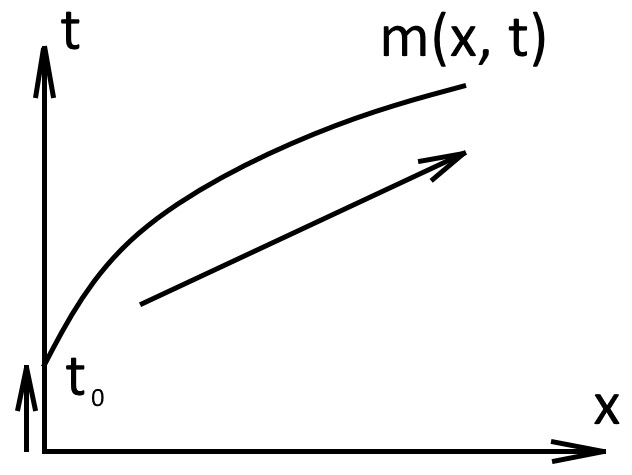
\includegraphics[width=7cm]{characteristics_solution_scheme.jpg}}
\caption{Схема решения методом характеристик.}
\label{fig:image1}
\end{figure}

\par В системе, которую мы уже писали раньше, заменим производную по времени производной по координате, что справедливо, поскольку мы находимся на характеристике.

\begin{equation*}
\begin{cases}

\d \frac{dm}{dx} &= \d \frac{m+\Phi(x)}{G(m)u_{0}}\\
&\\
\d \frac{dx}{dt}&= \d \frac{u_{0}}{m}\\
&\\
m_{t} &= -F(m)\alpha\\

\end{cases}
\end{equation*}

\par Запишем условия для нашей исходной задачи для функции $F(x)$ и граничные и начальные условия. Отсюда получается, что $\d G(x)=-\frac{1}{\gamma u_{0}}$, при $x=0$ концентрация частиц постоянна и равна $\alpha_{0}$, в начальный момент времени полагаем всюду пористость $m=m_{0} = const$.

\begin{equation*}
\begin{cases}

\d \frac{dm}{dx} = \d -\gamma (m+\Phi(x))\\
{}\\
\d \frac{dx}{dt}= \d \frac{u_{0}}{m}\\
{}\\
m_{t} = -\gamma u_{0}\alpha\\

\end{cases}
\end{equation*}

\par Получим решение в некотором параметрическом виде. Ход решения изображён на рис. 4. Сначала мы найдём, какая пористость будет на искомой характеристике при $x=0$ в момент времени $t = \hat{t}$. Решим первое уравнение в системе:

$$\frac{dm}{dx}=\gamma(m_{0}-m)$$
$$\frac{d(m_{0}-m)}{m_{0}-m}=-\gamma dx$$
$$ln(m_{0}-m)=-\gamma x + C$$
$$m_{0}-m = e^{c}e^{-\gamma x}$$
\par Теперь выразим $e^{c}$ через $m(\hat{t})$. На границе выполняется уравнение $m_{t}=-\alpha_{0}\gamma u_{0}$. Его решение имеет вид: 
$$m(x=0,t)=-\alpha_{0}\gamma u_{0}t+m_{0}$$
\par Значит, в момент времени $\hat{t}$ мы имеем пористость на входе в пласт, равную $m(x=0,\hat{t})=-\alpha_{0}\gamma u_{0}\hat{t}+m_{0}$. 
\par Используем его для нахождения произвольной постоянной:
$$m_{0}-m(x=0,\hat{t})= \alpha_{0}\gamma u_{0}\hat{t} = e^{c}$$
\par Получили выражение для $m(x,\hat{t})$:
$$m =m_{0} -\alpha_{0}\gamma u_{0}\hat{t}e^{-\gamma x}$$
\par Выразим $\hat{t}$, зная искомое решение (из которого мы получили $\Phi(x)$:
$$m_{0}-\gamma u_{0} \alpha_{0}\hat{t}=m_{0}-\gamma u_{0}\frac{t-x\frac{m_{0}}{u_{0}}}{1-\frac{\alpha_{0}-1}{\alpha_{0}}e^{\gamma x}}$$
\par Выразим $\hat{t}$:
$$\hat{t}=\frac{e^{\gamma x}(t-x\frac{m_{0}}{u_{0}})}{\alpha_{0}-(\alpha_{0}-1)e^{\gamma x}}$$